\chapter{Netzwerklastverteilung}
\begin{figure}
    \centering
    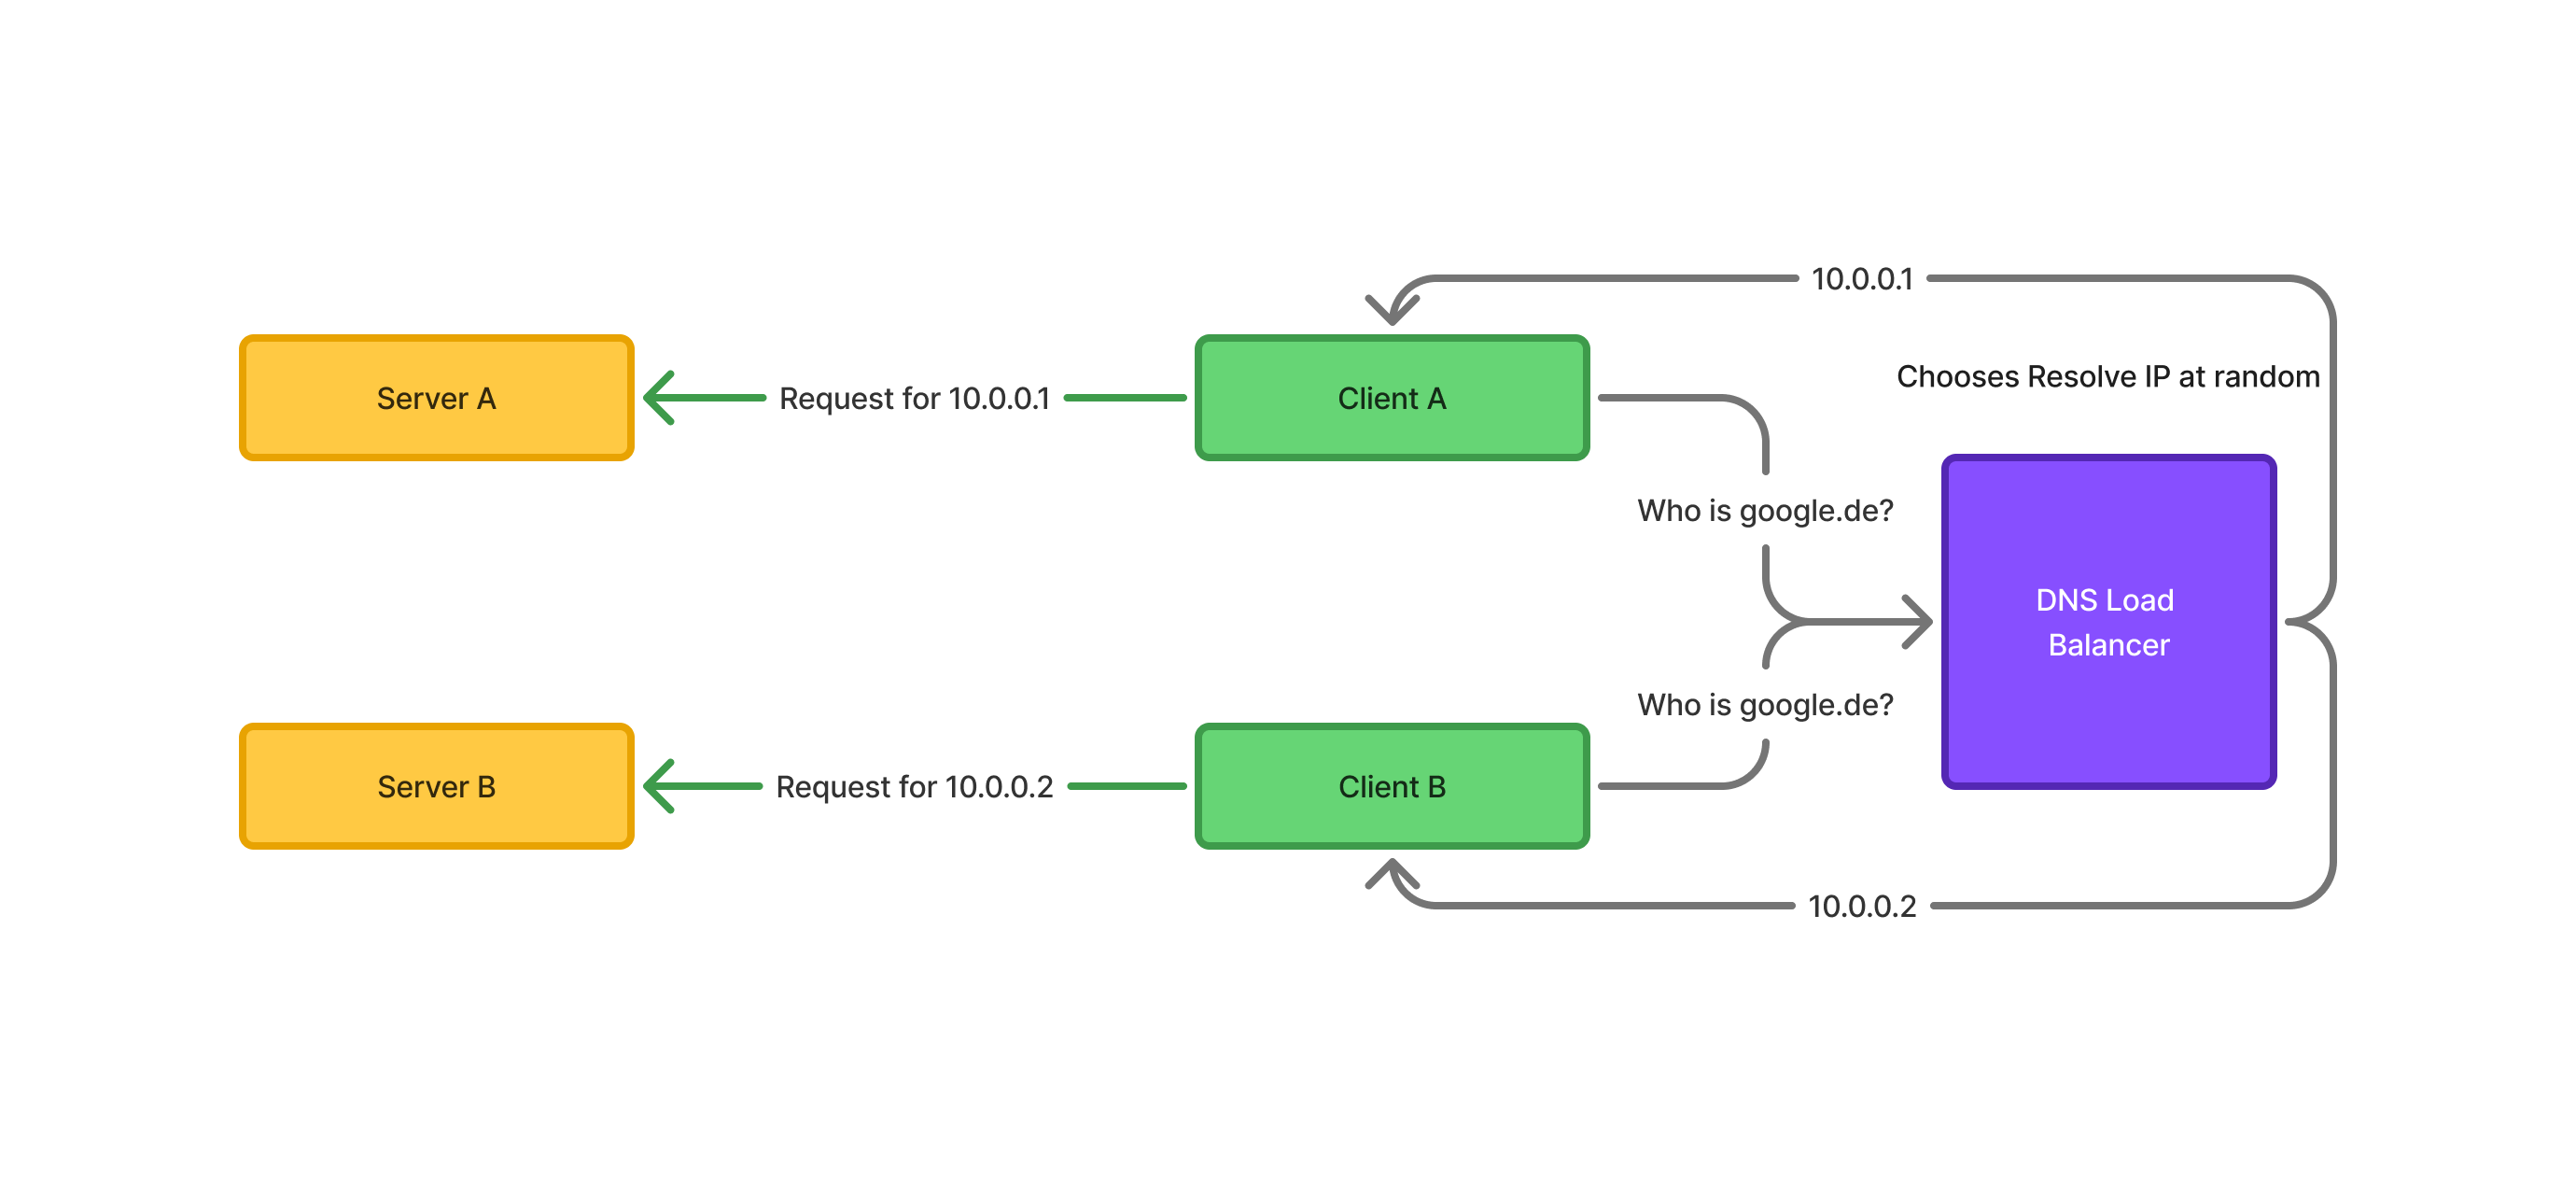
\includegraphics[width=1.1\linewidth]{images/DNS Loadbalancer(1).png}
    \caption{Aufbau eines DNS Loadbalancers}
    \label{fig:enter-label}
\end{figure}
Lastverteilung spielt in der Computerwissenschaft eine sehr wichtige Rolle. Das Problem wird immer dann interessant, wenn ein Computersystem an seine Grenzen der Bearbeitbarkeit gebracht wird. So wird auch bei Mehrkernprozessoren ein Algorithmus derart aufgeteilt, dass jeder Kern ein Teilproblem löst, welches nach Fertigstellung des Teilproblems mit den Ergebnissen der anderen Kerne zusammengesetzt wird. So lässt sich in vielen Fällen ein sehr bedeutender Speedup für bestimmte Algorithmen erreichen, indem der Algorithmus auf mehrere Recheneinheiten verteilt wird. \cite{lbtheory}

Betrachten wir nun Computerarchitekturen in Netzwerkumgebungen, so bilden wir eine Abstraktionsebene über den Mehrkernprozessoren. Nun ist es nicht mehr nur von Interesse, wie ein einzelner Prozessor das theoretische Problem bearbeitet, sondern es muss vielmehr betrachtet werden, wie sich besagtes Problem in einem Netzwerk aus Computern verhält. Mit dem Aufkommen des zivil und populär verfügbaren Internetanschlusses in den 90er Jahren ist vor allem die netzwerkbasierte Lastverteilung relevant. Die Kapazität eines einzelnen Computers, die Anfragen von Nutzern aus dem Internet zu verarbeiten, ist schnell erreichbar, sobald die Nachfrage auf Nutzerseite groß ist. So entstanden alsbald in den 90ern Ideen, wie es dennoch möglich ist, hochskalierende Anfrageraten zu beantworten. 

Im Folgenden wird ein Überblick über die klassischen bis hin zu den modernen Ansätzen der Lastverteilung in Rechnernetzen gegeben.

\section{Entstehung}

Wie bereits erwähnt, ist mit dem Aufkommen des Internets parallel das Interesse an Möglichkeiten der Lastverteilung gestiegen. Noch bevor dazu dedizierte Maschinen oder Anwendungen entwickelt wurden, gab es Ansätze, das Problem zu lösen. Dabei wurde der Aufbau des DNS-Systems genutzt. Wenn eine bestimmte URL von einem Client-Rechner angefordert wird, so wird zunächst eine Anfrage, in der die gesuchte URL steht, an einen DNS-Server geschickt. Dieser schlägt daraufhin nach, ob ihm die URL bekannt ist. Sollte dies der Fall sein, so schickt er ein Paket mit der entsprechenden IP-Adresse zurück an den Client-Rechner. \cite{hong2006dns} Dabei lässt sich nun auf ganz einfache Art und Weise die Last verteilen. Der DNS-Server hat, wie in Abbildung 5.1 zu sehen, nicht nur eine IP-Adresse für einen Server hinterlegt, sondern mehrere, aus denen er nun aus einem eigens dafür implementierten Algorithmus wählen kann, welche IP an den Client zurückgesendet wird. So konnte damals bereits mit einfachen Mitteln Last verteilt werden. 

Allerdings bringt dieser Ansatz natürlich eine Reihe von Problemen mit sich. So kann der DNS-Server den aktuellen Status der Backend-Server nicht kennen. Sollte einer der Backend-Server offline sein, so wird weiterhin seine IP an die Clients gesendet und somit als funktionierendes Backend propagiert. Außerdem lässt ein DNS-Server keine intelligente Lastverteilung zu. Bei dieser verbesserten Form der Lastverteilung werden die Prozessorauslastung, Speichernutzung oder anderweitige Ressourcenstatistiken verwendet, um eine Entscheidung darüber zu fällen, welches Backend noch weitere Anfragen bearbeiten kann. Außerdem müsste der Client den entsprechenden DNS-Server standardmäßig konfiguriert haben. Dies ist aber nicht zwingend gewährleistet.

\section{Hardwarelastverteiler}
Zum Ende der 90er Jahre hin zum Beginn der 2000er entwickelten eine Reihe von Herstellern hardwarebasierte Lastverteilungslösungen. Nennenswerte Hersteller sind hierbei F5-Networks mit \textbf{BIG-IP} (siehe Abbildung 5.2) aber auch Cisco oder Citrix. Bei diesen Geräten kamen auch erstmalig ASICs zum Einsatz. Grund dafür war die Tatsache, dass damalige Prozessoren bei weitem nicht schnell genug waren, um große Datenströme zu verarbeiten. Außerdem boten die damaligen Geräte zusätzliche Funktionalitäten an. Darunter waren grafische Nutzeroberflächen oder integrierte Backend Health Checks. \cite{bigip} Die damaligen ASICs fokussierten sich damals vor allem auf L4-Paket-Forwarding. Außerdem wurden derartige Geräte meist als eine Art Komplettlösung für sämtliche Aufgaben des Datenverkehrs vermarktet. So wurde auf selbigen Geräten meistens eine Firewall mit angeboten, wodurch auch sicherheitstechnische Funktionen wie Distributed Denial of Service Attacken bekämpft werden konnten. All diese Funktionen konnten mithilfe von Logging untersucht und analysiert werden. Außerdem konnten einige Hardwarelastverteiler auch an Anwendungen angepasst werden, sodass zusätzlich eine L7-Lastverteilung möglich wurde.
\begin{figure}
    \centering
    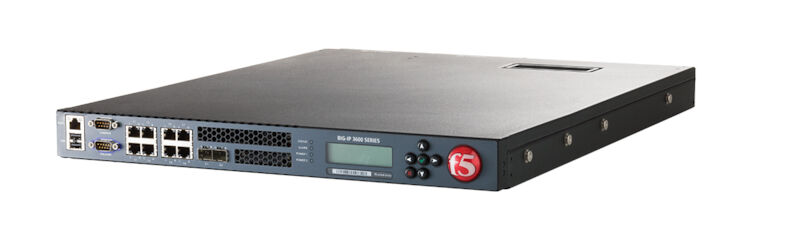
\includegraphics[width=1\linewidth]{images/s-l1600.jpg}
    \caption{BIG-IP von F5-Networks}
    \label{fig:enter-label}
\end{figure}
\section{Softwarelastverteiler}
Softwarelastverteiler unterscheiden sich deutlich von den Hardwarelastverteilern in dem Punkt, dass bei softwarebasierter Lastverteilung keine spezialisierte Hardware in Form von ASICs oder FPGAs zum Einsatz kommt. Es werden lediglich Programme auf Servern ausgeführt, deren Funktion es ist, den Netzwerkverkehr zu steuern. Wie im vorherigen Absatz beschrieben ist dies nur aufgrund der Entwicklungen im Bereich der Hardware der letzten zwei Jahrzehnte möglich geworden. Während dieser Zeit wurden gängige Prozessoren nicht nur um Rechenkerne erweitert, sondern erhielten außerdem größeren Cache und schnellere Anbindungen an sonstige Ein- und Ausgabeeinheiten. Außerdem lassen sich softwarebasierte Lastverteiler deutlich besser in moderne, meist VM-betriebene Netzwerkumgebungen integrieren. Die Natur eines anwendungsbasierten Lastverteilers bietet die Möglichkeit, genaue anwendungsfallspezifische Modifikationen vorzunehmen, womit eine kompakte Integration in ein System vorgenommen werden kann. \cite{softwarelb} So entstanden eine Menge von nennenswerten Anwendungen, die sich eine Lösung von softwarebasierter Lastverteilung zum Ziel gesetzt haben. Die wohl bekanntesten aktuellen Vertreter dieser Klasse sind Programme wie HAProxy, Nginx und mod\_proxy von Apache. \cite{soni2016load} Außerdem ist ebenfalls an der Universität Potsdam im Rahmen der Masterarbeit von Phillip Ungrund der Katran Lastverteiler  in einem ähnlichen Testszenario untersucht worden. Diese Messreihe ist sehr gut mit dem XenoFlow vergleichbar, da in Phillip Ungrunds Messungen ebenfalls DNS-Pakete verwendet wurden \cite{ungrund}. 
\section{Kubernetes und moderne Load Balancer}
Kubernetes ist eine moderne Container-Runtime, welche im Gegensatz zu klassischem Docker oder Podman nicht nur auf einem Rechner laufen kann, sondern gleich eine Netzwerkabstraktion mit sich bringt. In dieser werden mehrere Computer zu einem Kubernetes-Cluster zusammengefasst und können mittels dedizierter Control-Plane-Knoten kontrolliert werden. In solch einer Umgebung wird fast vollständig über REST-APIs kommuniziert. Anwendungen werden in solch einem Cluster in feingranulare Microservices heruntergebrochen. Ziel eines solchen Ansatzes ist es, die Teile eines komplexen Systems einzeln wartbar zu machen, aber auch Skalierfähigkeit zu erhalten. Grundsätzlich wird in Kubernetes-Clustern stets empfohlen, den einzelnen Microservices möglichst wenig State zu geben. Damit soll garantiert werden, dass die Provisionierung von Kubernetes übernommen werden kann. Dinge wie Replikas und redundante Anwendungen können so von Kubernetes bereitgestellt werden. \cite{vasireddy2023kubernetes}

In besagter Kubernetes-Architektur werden Ressourcen typisiert. So werden Container in Ressourcen vom Typ \textbf{Pod} ausgeführt. Diese sind meistens ebenfalls ein Teil einer abstrakteren Ressource namens \textbf{Deployment}, in der mehrere Pods zusammengefasst werden können. Damit nun ein solches Deployment von außerhalb des Kubernetes Clusters erreichbar ist, muss eine Ressource vom Typ \textbf{Service} definiert werden. Solch ein Service kann wiederum unterschiedliche Arten haben. Ist die Art des Services \textbf{LoadBalancer} so wird an einen eventuellen Cloud Provider wie GKE (Google), AWS (Amazon) oder Azure (Microsoft) kommuniziert, dass eine Lastverteilungs-IP-Adresse bereitgestellt werden soll, die auf den verknüpften Service zeigen soll. Dieser Service zeigt wiederum auf das Deployment, in dem entsprechend der gesuchte Endpunkt für die Kommunikation liegt. 

In einem solchen Umfeld ist es somit den Cloud-Providern überlassen, wie sie die Lastverteilung genau vornehmen. Damit können alle oben genannten Ansätze zum Einsatz kommen. Der im Rahmen dieser Arbeit implementierte Load Balancer eignet sich in einem solchen Szenario sehr gut, da er auf der Netzwerkkarte des Providers in den für die Lastverteilung bestimmten Servern ausgeführt werden kann.